\achapter{33}{The Dimension of a Vector Space} \label{sec:dimension}

\vspace*{-17 pt}
\framebox{
\parbox{\dimexpr\linewidth-3\fboxsep-3\fboxrule}
{\begin{fqs}
\item What is a finite dimensional vector space? 
\item What is the dimension of a finite dimensional vector space? What important result about bases of finite dimensional vector spaces makes dimension well-defined?
\item What must be true about any linearly independent subset of $n$ vectors in a vector space with dimension $n$? Why?
\item What must be true about any subset of $n$ vectors in a vector space with dimension $n$ that spans the vector space? Why?
\end{fqs}}}% \hspace*{3 pt}}
 
\vspace*{13 pt}

\csection{Application: Principal Component Analysis}

The discipline of statistics is based on the idea of analyzing data. In large data sets it is usually the case that one wants to understand the relationships between the different data in the set. This can be difficult to do when the data set is large and it is impossible to visually examine the data for patterns. Principal Component Analysis (PCA) is a tool for identifying and representing underlying patterns in large data sets, and PCA has been called one of the most important and valuable linear algebra tools for statistical analysis. PCA is used to transform a collection of variables into a (usually smaller) number of uncorrelated variables called principal components. The principal components form the most meaningful basis from which to view data by removing extraneous information and revealing underlying relationships in the data. This presents a framework for how to reduce a complex data set to a lower dimension while retaining the important attributes of the data set.  The output helps the experimenter determine which dynamics in the data are important and which can be ignored. 

\csection{Introduction}

In Section \ref{sec:bases_dimension} we learned that any two bases for a subspace of $\R^n$ contain the same number of vectors. This allowed us to define the dimension of a subspace of $\R^n$. In this section we extend the arguments we made in Section \ref{sec:bases_dimension} to arbitrary vector spaces and define the dimension of a vector space. 

\begin{pa} \label{pa:5_c} The main tool we used to prove that any two bases for a subspace of $\R^n$ must contain the same number of elements was Theorem \ref{thm:3_d_1}. In this preview activity we will show that the same argument can be used for vector spaces. More specifically, we will prove a special case of the following theorem generalizing Theorem \ref{thm:3_d_1}.

\begin{theorem} \label{thm:5_c_1} If $V$ is a vector space with a basis $\CB = \{\vv_1, \vv_2, \ldots, \vv_k\}$ of $k$ vectors, then any subset of $V$ containing more than $k$ vectors is linearly dependent.
\end{theorem} 

Suppose $V$ is a vector space with basis $\CB = \{\vv_1, \vv_2\}$. Consider the set $U=\{\vu_1, \vu_2, \vu_3\}$ of vectors in $V$. We will show that $U$ is linearly dependent using a similar approach to the Preview Activity \ref{pa:3_d}.

\be

\item What vector equation involving $\vu_1, \vu_2, \vu_3$ do we need to solve to determine linear independence/dependence of these vectors? Use $x_1, x_2, x_3$ for coefficients.

\item Since $\CB$ is a basis of $V$, it spans $V$. Using this information, rewrite the vectors $\vu_i$ in terms of $\vv_j$ and substitute into the above equation to obtain another equation in terms of $\vv_j$.

\item Since $\CB$ is a basis of $V$, the vectors $\vv_1, \vv_2$ are linearly independent. Using the equation in the previous part, determine what this means about the coefficients $x_1, x_2, x_3$.

\item Express the conditions on $x_1, x_2, x_3$ in the form of a matrix-vector equation. Explain why there are infinitely many solutions for $x_i$'s and why this means the vectors $\vu_1, \vu_2, \vu_3$ are linearly dependent.

\ee


\end{pa}



\csection{Finite Dimensional Vector Spaces}


Theorem \ref{thm:5_c_1} shows that if sets $\CB_1$ and $\CB_2$ are finite bases for a vector space $V$, which are linearly independent by definition, then each cannot contain more elements than the other, so the number of elements in each basis must be equal. 

\begin{theorem} \label{thm:5_c_2} If a non-trivial vector space $V$ has a basis of $n$ vectors, then every basis of $V$ contains exactly $n$ vectors.
\end{theorem}


Theorem \ref{thm:5_c_2} states that if a vector space $V$ has a basis with a finite number of vectors, then the number of vectors in a basis for that vector space is a well-defined number. In other words, the number of vectors in a basis is an \emph{invariant} of the vector space. This important number is given a name.


\begin{definition} A \textbf{finite-dimensional}\index{vector space!finite dimensional} vector space is a vector space that can be spanned by a finite number of vectors. The \textbf{dimension}\index{vector space!dimension} of a non-trivial finite-dimensional vector space is the number of vectors in a basis for $V$. The dimension of the trivial vector space is defined to be 0.
\end{definition}


We denote the dimension of a finite dimensional vector space $V$ by $\dim(V)$.


Not every vector space is finite dimensional. We have seen, for example, that the vector space $\pol$ of all polynomials, regardless of degree, is not a finite-dimensional vector space. In fact, the polynomials
\[1, t, t^2, \ldots, t^n, \ldots\]
are linearly independent, so $\pol$ has an infinite linearly independent set and therefore has no finite basis. A vector space that has an infinite basis is called an \emph{infinite dimensional} vector space. 


\begin{activity} \label{act:5_c_1} Since columns of the $n \times n$ identity matrix span $\R^n $ and are linearly independent, the columns of $I_n$ form a basis for $\R^n$ (the standard basis). Consequently, we have that $\dim(\R^n) = n$. In this activity we determine the dimensions of other familiar vector spaces. Find the dimensions of each of the indicated vector spaces. Verify your answers.
	\ba
	\begin{minipage}{1.5in}
	\item $\pol_1$
	\end{minipage}
	\begin{minipage}{1.5in}
	\item $\pol_2$
	\end{minipage}
	\begin{minipage}{1.5in}
	\item $\pol_n$
	\end{minipage}
	
	\begin{minipage}{1.5in}
	\item $\M_{2 \times 3}$
	\end{minipage}
	\begin{minipage}{1.5in}
	\item $\M_{3 \times 4}$
	\end{minipage}
	\begin{minipage}{1.5in}
	\item $\M_{k \times n}$
	\end{minipage}

\ea


\end{activity}

Finding the dimension of a finite-dimensional vector space amounts to finding a basis for the space. 

\begin{activity} \label{act:5_c_2}  Let $W = \{(a+b) + (a-b)t + (2a+3b)t^2 \mid a, b \text{ are scalars}\}$. 
	\ba
	\item Find a finite set of polynomials in $W$ that span $W$. 


	\item Determine if the spanning set from part (a) is linearly independent or dependent. Clearly explain your process. 
		
	
	\item What is $\dim(W)$? Explain.
	
	\ea
	
\end{activity}

\csection{The Dimension of a Subspace}

Every subspace of a finite-dimensional vector space is a vector space, and since a subspace is contained in a vector space it is natural to think that the dimension of a subspace should be less than or equal to the dimension of the larger vector space. We verify that fact in this section.


\begin{activity} \label{act:5_c_3} Let $V$ be a finite dimensional vector space of dimension $n$ and let $W$ be a subspace of $V$. Explain why $W$ cannot have dimension larger than $\dim(V)$, and if $W \neq V$ then $\dim(W) < \dim(V)$. (Hint: Use Theorem \ref{thm:5_c_1}.)

\end{activity}


\csection{Conditions for a Basis of a Vector Space}

There are two items we need to confirm before we can state that a subset $\CB$ of a subspace $W$ of a vector space is a basis for $W$: the set $\CB$ must be linearly independent and span $W$. We can reduce the amount of work it takes to show that a set is a basis if we know the dimension of the vector space in advance. 


\begin{activity} \label{act:5_c_5} Let $W$ be a subspace of a vector space $V$ with $\dim(W) = k$. We know that every basis of $W$ contains exactly $k$ vectors. 
	\ba
	\item Suppose that $S$ is a subset of $W$ that contains $k$ vectors and is linearly independent. In this part of the activity we will show that $S$ must span $W$.
		\begin{enumerate}[i.]
		\item Suppose that $S$ does not span $W$. Explain why this implies that $W$ contains a set of $k+1$ linearly independent vectors. 		

	\item Explain why the result of i tells us that $S$ is a basis for $W$. 

	\end{enumerate}

\item Now suppose that $S$ is a subset of $W$ with $k$ vectors that spans $W$. In this part of the activity we will show that $S$ must be linearly independent.
	\begin{enumerate}[i.]
	\item Suppose that $S$ is not linearly independent. Explain why we can then find a proper subset of $S$ that is linearly independent but has the same span as $S$. 


	\item Explain why the result of i tells us that $S$ is a basis for $W$. 


	\end{enumerate}

\ea

\end{activity}



The result of Activity \ref{act:5_c_5} is summarized in the following theorem (compare to Theorem \ref{thm:3_d_basis_properties}).



\begin{theorem} Let $W$ be a subspace of dimension $k$ of a vector space $V$ and let $S$ be a subset of $W$ containing exactly $k$ vectors.
\begin{enumerate}
\item If $S$ is linearly independent, then $S$ is a basis for $W$.
\item If $S$ spans $W$, then $S$ is a basis for $W$.
\end{enumerate}
\end{theorem}

\csection{Examples}

\ExampleIntro

\begin{example} Find a basis and dimension for each of the indicated subspaces of the given vector spaces.
	\ba
	\item $\{a+b(t+t^2) : a, b \in \R\}$ in $\pol_2$
	
	\item $\Span\left\{1, \frac{1}{1+x^2}, \frac{2+x^2}{1+x^2}, \arctan(x)\right\}$ in $\F$
	
	\item $\{p(t) \in \pol_n : p(-t) = p(t)\}$ in $\pol_4$ (The polynomials with the property that $p(-t) = p(t)$ are called \emph{even} polynomials.)
	
	\ea

\ExampleSolution
	\ba
	\item Let $W = \{a+b(t+t^2) : a, b \in \R\}$. Every element in $W$ has the form 
	\[a+b(t+t^2) = a(1) + b(t+t^2).\]
	So $W = \Span\{1, t+t^2\}$. Since neither $1$ nor $t+t^2$ is a scalar multiple of the other, the set $\{1, t+t^2\}$ is linearly independent. Thus, $\{1, t+t^2\}$ is a basis for $W$ and $\dim(W) = 2$. 
	
	\item Let $W = \Span\left\{1, \frac{1}{1+x^2}, \frac{2+x^2}{1+x^2}, \arctan(x)\right\}$. To find a basis for $W$, we find a linearly independent subset of $\left\{1, \frac{1}{1+x^2}, \frac{2+x^2}{1+x^2}, \arctan(x)\right\}$.  Consider the equation
	\[c_1 (1) + c_2\left(\frac{1}{1+x^2}\right) + c_3\left(\frac{2+x^2}{1+x^2}\right) + c_4 \arctan(x) = 0.\]
	To find the weights $c_i$ for which this equality of functions holds, we use the fact that the we must have equality for every $x$. So we pick four different values for $x$ to obtain a linear system that we can solve for the weights. Evaluating both sides of the equation at $x=0$, $x=1$, $x=-1$, and $x=2$ yields the equations
	\begin{alignat*}{5}
{}c_1 	&{}+{} 	&{}c_2		&{}+{}	&{2}c_3	&{}	&{}		&= \ &0&{} \\
{}c_1 	&{}+{} 	&{\frac{1}{2}}c_2	&{}+{}		&{\frac{3}{2}}c_3		&{}+{}	&{\frac{\pi}{4}}c_4		&= \ &0&{} \\
{}c_1 	&{}+{} 	&{\frac{1}{2}}c_2	&{}+{}		&{\frac{3}{2}}c_3		&{}-{}	&{\frac{\pi}{4}}c_4		&= \ &0&{} \\
{}c_1 	&{}+{} 	&{\frac{1}{5}}c_2	&{}+{}		&{\frac{6}{5}}c_3		&{}+{}	&{\arctan(2)}c_4		&= \ &0&{.} \\
\end{alignat*}
The reduced row echelon form of the coefficient matrix 
\[\left[ \renewcommand{\arraystretch}{1.4} \begin{array}{cccr} 1&1&2&0 \\ 1&\frac{1}{2}&\frac{3}{2}&\frac{\pi}{4} \\ 1&\frac{1}{2}&\frac{3}{2}&-\frac{\pi}{4} \\ 1&\frac{1}{5}&\frac{6}{5}&\arctan(2) \end{array} \right]\]
is 
$\left[ \begin{array}{cccc} 1&0&1&0 \\ 0&1&1&0 \\ 0&0&0&1 \\ 0&0&0&0 \end{array} \right]$. The general solution to this linear system is $c_1 = c_2 = -c_3$ and $c_4 = 0$. Notice that 
\[(-1)(1) + (-1)\left( \frac{1}{1+x^2}\right) + \frac{2+x^2}{1+x^2} = 0\]
or
\[ \frac{2+x^2}{1+x^2} = 1 + \left( \frac{1}{1+x^2}\right),\]
so $\frac{2+x^2}{1+x^2}$ is a linear combination of the other vectors. The vectors corresponding to the pivot columns are linearly independent, so it follows that $1$, $\frac{1}{1+x^2}$, and $\arctan(x)$ are linearly independent. We conclude that $\left\{1, \frac{1}{1+x^2},  \arctan(x)\right\}$ is a basis for $W$ and $\dim(W) = 3$. 
	
	\item Let $W = \{p(t) \in \pol_n : p(-t) = p(t)\}$ in $\pol_4$. Let $p(t) \in W$ and suppose that $p(t) = a_0 + a_1t+a_2t^2+a_3t^3+a_4t^4$.  Since $p(-t)=p(t)$, we must have $p(1) = p(-1)$ and $p(3) = p(-3)$. Since $p(1) = p(-1)$, it follows that 
	\[a_0+a_1+a_2+a_3+a_4 = a_0-a_1+a_2-a_3+a_4\]
	or
	\[a_1+a_3 = 0.\]
	Similarly, the fact that $p(3) = p(-3)$ yields the equation
	\[a_0+3a_1+9a_2+27a_3+81a_4 = a_0-3a_1+9a_2-27a_3+81a_4\]
	or
	\[a_1+9a_3 = 0.\]
	The reduced row echelon form of the coefficient matrix of system $a_1+a_3 = 0$ and $a_1+9a_3 = 0$ is $I_2$, so it follows that $a_1=a_3=0$. Thus, $p(t) = a_0 + a_2t^2+a_4t^4$ and so $W = \Span\{1, t^2, t^4\}$. Equating like terms in the equation 
	\[c_1(1) + c_2(t^2) + c_3(t^4) = 0\]
	yields $c_1=c_2=c_3=0$. We conclude that $\{1,t^2,t^4\}$ is linearly independent and is therefore a basis for $W$. Thus, $\dim(W) = 3$. 

As an alternative solution, notice that $p(t) = t$ is not in $W$. So $W \neq V$ and we know that $\dim(W) < \dim(V)$. Since $1$, $t^2$, and $t^4$ are in $W$, we can show as above that $1$, $t^2$, and $t^4$ are linearly independent. We can conclude that $\dim(W)=3$ since it cannot be $4$. 
	\ea
	
\end{example}


\begin{example} Let $U_{n \times n}$ be the set of all $n \times n$ upper triangular matrices. Recall that a matrix $A = [a_{ij}]$ is upper triangular if $a_{ij} = 0$ whenever $i > j$. That is, a matrix is upper triangular if all entries below the diagonal are 0. 
	\ba
	\item Show that $U_{n \times n}$ is a subspace of $\M_{n \times n}$. 

	\item Find the dimensions of $U_{2 \times 2}$ and $U_{3 \times 3}$. Explain. Make a conjecture as to what $\dim(U_{n \times n})$ is in terms of $n$.
	 
	 \ea

\ExampleSolution
\ba
\item Since the $n \times n$ zero matrix $0_{n \times n}$ has all entries equal to 0, it follows that $0_{n \times n}$ is in $U_{n \times n}$.  Let $A = [a_{ij}]$ and $B = [b_{ij}]$ be in $U_{n \times n}$, and let $C = [c_{ij}] = A+B$. Then $c_{ij} = a_{ij} + b_{ij} = 0 + 0$ when $i > j$. So $C$ is an upper triangular matrix and $U_{n \times n}$ is closed under addition. Let $c$ be a scalar. The $ij$th entry of $cA$ is $ca_{ij} = c(0) = 0$ whenever $i > j$. So $cA$ is an upper triangular matrix and $U_{n \times n}$ is closed under multiplication by scalars. We conclude that $U_{n \times n}$ is a subspace of $\M_{n \times n}$. 

\item  Let $M_{11} = \left[ \begin{array}{cc} 1&0 \\ 0&0 \end{array} \right]$, $M_{12} = \left[ \begin{array}{cc} 0&1 \\ 0&0 \end{array} \right]$, and $M_{22}=\left[ \begin{array}{cc} 0&0 \\ 0&1 \end{array} \right]$. We will show that $S = \{M_{11}, M_{12}, M_{22}\}$ is a basis for $U_{2 \times 2}$.  Consider the equation 
\[x_1M_{11} + x_2M_{12} + x_3 M_{22} = 0.\]
Equating like entries shows that $x_1 = x_2 = x_3 = 0$, and so $S$ is linearly independent. If $\left[ \begin{array}{cc} a&b \\ 0&c \end{array} \right]$ is in $U_{2 \times 2}$, then 
\[\left[ \begin{array}{cc} a&b \\ 0&c \end{array} \right] = aM_{11} + bM_{12} + cM_{22}\]
and so $S$ spans $U_{2 \times 2}$. Thus, $S$ is a basis for $U_{2 \times 2}$ and so $\dim(U_{2 \times 2}) = 3$. 

Similarly, for the $3 \times 3$ case let $M_{ij}$ for $i \leq j$ be the $3 \times 3$ matrix with a 1 in the $ij$ position and 0 in every other position. Let 
\[S = \{M_{11}, M_{12}, M_{13}, M_{22}, M_{23}, M_{33}\}.\]
Equating corresponding entries shows that if 
\[x_1M_{11} +  x_2M_{12} + x_3M_{13} + x_4 M_{22}+ x_5 M_{23} + x_6M_{33} = 0,\]
then $x_1 = x_2 = x_3 = x_4 = x_5 = x_6 = 0$. So $S$ is a linearly independent set. If $A = [a_{ij}]$ is in $U_{3 \times 3}$, then $A = \sum_{i \geq j} a_{ij}M_{ij}$ and $S$ spans $U_{3 \times 3}$. We conclude that $S$ is a basis for $U_{3 \times 3}$ and $\dim(U_{3 \times 3}) = 6$. 

In general, for an $n \times n$ matrix, the set of matrices $M_{ij}$, one for each entry on and above the diagonal, is a basis for $U_{n \times n}$. There are $n$ such matrices for the entries on the diagonal. The number of entries above the diagonal is equal to half the total number of entries ($n^2$) minus half the number of entries on the diagonal ($n$). So there is a total of $\frac{n^2-n}{2}$ such matrices for the entries above the diagonal. Therefore, 
\[\dim(U_{n \times n}) = n+\frac{n^2-n}{2} = \frac{n^2+n}{2}.\] 

%In general, if $M_{ij}$ for $i \leq j$ is the $n \times n$ matrix with a 1 in the $ij$ position and 0 in every other position, the set $S = \{M_{ij}\}_{i \geq j}$ is a basis for $U_{n \times n}$. If $j =1$,  then there are $n$ values of $i$ that are greater than or equal to $j$ and less than or equal to $n$. If $j=2$, then there are $n-1$ values of $i$ that are greater than or equal to $j$ and less than or equal to $n$. In general, there are $n-(j-1)$ values of $i$ that are between $j$ and $n$.  So there are 
%\[\sum_{j=1}^n n-(j-1) = n^2+n-\sum_{j=1}^n j = n(n+1) - \frac{n(n+1)}{2} = \frac{n(n+1)}{2}\]
%of these matrices in total. Therefore, $\dim(U_{n \times n}) = \frac{n(n+1)}{2}$. 

\ea

\end{example}



\csection{Summary}

\begin{itemize}
\item A finite dimensional vector space is a vector space that can be spanned by a finite set of vectors.
\item We showed that any two bases for a finite dimensional vector space \emph{must} contain the same number of vectors. Therefore, we can define the \emph{dimension} of a finite dimensional vector space $V$ to be the number of vectors in any basis for $V$.
\item If $V$ is a vector space with dimension $n$ and $S$ is any linearly independent subset of $V$ with $n$ vectors, then $S$ is a basis for $V$. Otherwise, we could add vectors to $S$ to make a basis for $V$ and then $V$ would have a basis of more than $n$ vectors. 
\item If $V$ is a vector space with dimension $n$ and $S$ is any subset of $V$ with $n$ vectors that spans $V$, then $S$ is a basis for $V$. Otherwise, we could remove vectors from $S$ to obtain a basis for $V$ and then $V$ would have a basis of fewer than $n$ vectors. 
\item For any finite dimensional space $V$ and a subspace $W$ of $V$, $\dim(W)\leq \dim(V)$.
%\item The rank of a matrix is the dimension of the column space of the matrix and the nullity of a matrix is the dimension of the null space of a matrix. The Rank-Nullity Theorem says that the sum of the rank and nullity of a matrix is equal to the number of columns of the matrix.
%\item If $V$ is an $n$-dimensional vector space with a basis $\CB$ of vectors $\vv_1$, $\vv_2$, $\ldots$, $\vv_n$, then the coordinate transformation $T$ from $V$ to $\R^n$ preserves linear combinations and is one-to-one and onto. So $T$ provides an identification of $V$ with $\R^n$. 
%\item Coordinate transformations allow us to use our knowledge of matrices to answer important questions in vector spaces by transferring the questions from a vector space into $\R^n$ using a coordinate transformation. 
\end{itemize}

\csection{Exercises}
\be


\item Let $W = \Span\{ 1+t^2, 2+t+2t^2+t^3, 1+t+t^3, t-t^2+t^3\}$ in $\pol_3$. Find a basis for $W$. What is the dimension of $W$?

\item Let $A = \left[ \begin{array}{cc} 1&2\\1&0 \end{array} \right]$ and $B = \left[ \begin{array}{cr} 1&0\\1&-1 \end{array} \right]$.
	\ba
	\item Are $A$ and $B$ linearly independent or dependent? Verify your result.
	\item Extend the set $S = \{A,B\}$ to a basis for $\M_{2 \times 2}$. That is, find a basis for $\M_{2 \times 2}$ that contains both $A$ and $B$. 
	\ea
	
	

\item Let $A = \left[ \begin{array}{ccc} 1&2&0 \\ 3&0&2 \end{array} \right]$, $B = \left[ \begin{array}{rcc} -1&1&1 \\ 2&4&0 \end{array} \right]$, $C= \left[ \begin{array}{crr} 5&1&-3 \\ 0&-12&4 \end{array} \right]$, $D = \left[ \begin{array}{crr} 5&4&-2 \\ 5&-8&6 \end{array} \right]$, and $E = \left[ \begin{array}{rcc} 2&0&0 \\ -2&0&1 \end{array} \right]$ in $\M_{2 \times 3}$ and let $S = \left\{ A, B, C, D, E \right\}$. 
	\ba
	\item Is $S$ a basis for $\M_{2 \times 3}$? Explain.
	\item Determine if $S$ is a linearly independent or dependent set. Verify your result.
	\item Find a basis $\CB$ for $\Span \ S$ that is a subset of $S$ and write all of the vectors in $S$ as linear combinations of the vectors in $\CB$. 
	\item Extend your basis $\CB$ from part (c) to a basis $\M_{2 \times 3}$. Explain your method. 
	\ea

	
\item Determine the dimension of each of the following vector spaces.
	\ba
	\item $\Span\{2, 1+t, t^2\}$ in $\pol_2$
	\item The space of all polynomials in $\pol_3$ whose constant terms is 0. 
	\item $\Nul  \left[ \begin{array}{cc} 1&2 \\ 2&4 \end{array} \right] $
	\item $\Span\left\{ [1 \ 2 \ 0 \ 1 \ -1]^{\tr}, [0 \ 1 \ 1 \ 1 \ 0]^{\tr},  [0 \ 3 \ 2 \ 3 \ 0]^{\tr}, [-1 \ 0 \ 1 \ 1 \ 1]^{\tr}\right\}$ in $\R^5$  
	\ea
	
\item Let $W$ be the set of matrices in $\M_{2 \times 2}$ whose diagonal entries sum to 0. Show that $W$ is a subspace of $\M_{2 \times 2}$, find a basis for $W$, and then find $\dim(W)$. 

\item Show that if $W$ is a subspace of a finite dimensional vector space $V$, then any basis of $W$ can be extended to a basis of $V$.

\item Let $W$ be the set of all polynomials $a+bt+ct^2$ in $\pol_2$ such that $a+b+c = 0$. Show that $W$ is a subspace of $\pol_2$, find a basis for $W$, and then find $\dim(W)$. 

\item Suppose $W_1, W_2$ are subspaces in a finite-dimensional space $V$.
\ba
\item Show that it is not true in general that $\dim(W_1)+\dim(W_2) \leq \dim(V)$.

\item Are there any conditions on $W_1$ and $W_2$ that will ensure that $\dim(W_1)+\dim(W_2) \leq \dim(V)$? (Hint: See problem \ref{problem:disjoint_subspaces} in the previous section.)  

\ea

\item Suppose $W_1 \subseteq W_2$ are two subspaces of a finite-dimensional space. Show that if $\dim(W_1)=\dim(W_2)$, then $W_1=W_2$.

\item Suppose $W_1, W_2$ are both three-dimensional subspaces inside $\R^4$. In this exercise we will show that $W_1\cap W_2$ contains a plane. Let $\{\vu_1, \vu_2, \vu_3\}$ be a basis for $W_1$ and let $\{\vv_1, \vv_2, \vv_3\}$ be a basis for $W_2$.
\ba
\item If $\vv_1$, $\vv_2$, and $\vv_3$ are all in $W_1$, explain why $W_1 \cap W_2$ must contain a plane. 

\item Now we consider the case where not all of $\vv_1$, $\vv_2$, and $\vv_3$ are in $W_1$. Since the arguments will be the same, let us assume that $\vv_1$ is not in $W_1$. 

	\begin{enumerate}[i.]
	\item Explain why the set $\CS = \{\vu_1, \vu_2, \vu_3, \vv_1\}$ is a basis for $\R^4$. 
	
	\item Explain why $\vv_2$ and $\vv_3$ can be written as linear combinations of the vectors in $\CS$. Use these linear combinations to find two vectors that are in $W_1 \cap W_2$. Then show that these vectors span a plane in $W_1 \cap W_2$.
	
	\end{enumerate}
\ea

\item A magic matrix is an $n \times n$ matrix in which the sum of the entries along any row, column, or diagonal is the same. For example, the $3 \times 3$ matrix 
\[\left[ \begin{array}{rcc} 5&4&0 \\ -2&3&8 \\ 6&2&1 \end{array} \right]\]
is a magic matrix. Note that the entries of a magic matrix can be any real numbers. 
\ba
\item Show that the set of $n \times n$ magic matrices is a subspace of $\M_{n \times n}$. 

\item Let $V$ be the space of $3 \times 3$ magic matrices. Find a basis for $V$ and determine the dimension of $V$. 

\ea

\item Label each of the following statements as True or False. Provide justification for your response.
\ba
\item \textbf{True/False} The dimension of a finite dimensional vector space is the minimum number of vectors needed to span that space.

\item \textbf{True/False} The dimension of a finite dimensional vector space is the maximum number of linearly independent vectors that can exist in that space.

\item \textbf{True/False} If $n$ vectors span an $n$-dimensional vector space $V$, then these vectors form a basis of $V$.

\item \textbf{True/False} Any set of $n$ vectors form a basis in an $n$-dimensional vector space.

\item \textbf{True/False} Every vector in a vector space $V$ spans a one-dimensional subspace of $V$.

\item \textbf{True/False} Any set of $n$ linearly independent vectors in a vector space $V$ of  dimensional $n$ is a basis for $V$. 

\item \textbf{True/False} If $\{\vv_1, \vv_2, \ldots, \vv_k\}$ is linearly independent in $V$, then $\dim(V)\geq k$.

\item \textbf{True/False} If a set of $k$ vectors span $V$, then any set of more than $k$ vectors in $V$ is linearly dependent.

\item \textbf{True/False} If an infinite set of vectors span $V$, then $V$ is infinite-dimensional.

\item \textbf{True/False} If $W_1, W_2$ are both two-dimensional subspaces of a three dimensional vector space $V$, then $W_1\cap W_2\neq \{\vzero \}$.

\item \textbf{True/False} If $\dim(V)=n$ and $W$ is a subspace of $V$ with dimension $n$, then $W=V$.

%\item \textbf{True/False} Let $A$ be an $n \times n$ matrix with $r$ pivots, where $r$ is less than or equal to $n$.  If $\dim(\Col A) < n$, then $A$ is non-invertible.

%\item \textbf{True/False} Let $A$ be an $n \times n$ matrix with $r$ pivots, where $r$ is less than or equal to $n$. If $\dim(\Nul A) = 0$, then $A$ is invertible.


\ea

\ee


\csection{Project: Understanding Principal Component Analysis}

Suppose we were to film an experiment involving a ball that is bouncing up and down. Naively, we set up several cameras to follow the process of the experiment from different perspectives and collect the data. All of this data tells us something about the bouncing ball, but there may be no perspective that tells us an important piece of information -- the axis along which the ball bounces. The question, then, is how we can extract from the data this important piece of information. Principal Component Analysis (PCA) is a tool for just this type of analysis. 


\begin{table}[ht]
\begin{center}
\begin{tabular}{lcccccccccc} 
State			&$1$	 &$2$ &$3$ &$4$ &$5$ &$6$ &$7$ &$8$ &$9$ &$10$ \\ \hline
EBRW		&$595$ &$540$ &$522$ &$508$ &$565$ &$512$ &$643$ &$574$ &$534$ &$539$ \\
Math			&$571$ &$536$ &$493$ &$493$ &$554$ &$501$ &$655$ &$566$ &$534$ &$539$ 
\end{tabular}
\caption{SAT data.}
\label{T:PCA_SAT_2}
\end{center}
\end{table}
We will use an example to illustrate important concepts we will need. To realistically apply PCA we will have much more data than this, but for now we will restrict ourselves to only two variables so that we can visualize our results. Table \ref{T:PCA_SAT_2} presents information from ten states on two attributes related to the SAT -- Evidence-Based Reading and Writing (EBRW) score and Math score. The SAT is made up of three sections: Reading, Writing and Language (also just called Writing), and Math. The The EBRW score is calculated by combining the Reading and Writing section scores -- both the Math and EBRW are scored on a scale of 200-800.
%https://blog.prepscholar.com/average-sat-scores-by-state-most-recent

Each attribute (Math, EBRW score) creates a vector whose entries are the student responses for that attribute. The data provides the average scores from participating students in each state. In this example we have two attribute vectors: 
\begin{align*}
\vx_1 &= [595 \ 540 \ 522 \ 508 \ 565 \ 512 \ 643 \ 574 \ 534 \ 539]^{\tr} \text{ and } \\
\vx_2 &= [571 \ 536 \ 493 \ 493 \ 554 \ 501 \ 655 \ 566 \ 534 \ 539]^{\tr}.
\end{align*}
 These vectors form the rows of a $2 \times 10$ matrix 
 \[X_0 = \left[ \begin{array}{c} \vx_1^{\tr} \\ \vx_2^{\tr} \end{array} \right] = \left[ \begin{array}{cccccccccc}  595&540&522&508&565&512&643&574&534&539
\\ 571&536&493&493&554&501&655&566&534&539
\end {array} \right] \]
that makes up our data set. A plot of the data is shown at left in Figure \ref{F:PCA_data_plot}, where the EBRW score is along the horizontal axis and the math score is along the vertical axis.
\begin{figure}[ht]
  \begin{center}
  \resizebox{!}{2.0in}{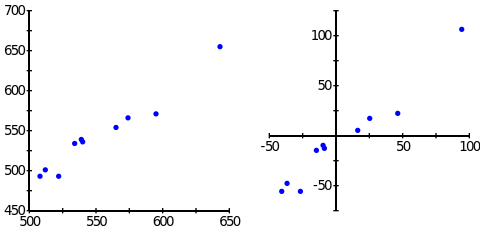
\includegraphics{PCA_data}} 
%\resizebox{!}{1.75in}{\includegraphics{PCA_2_original}} \hspace{0.5in} \resizebox{!}{1.75in}{\includegraphics{PCA_2_centered}} 
    \caption{Two views of the data set (EBRW horizontal, math vertical).}
    \label{F:PCA_data_plot}
  \end{center}
\end{figure}
The question we want to answer is, how do we represent our data set so that the most important features in the data set are revealed?  

\begin{pactivity} \label{act:PCA_centering} Before analyzing a data set there is often some initial preparation that needs to be made. Issues that have to be dealt with include the problem that attributes might have different units and scales. For example, in a data set with attributes about people, height could be measured in inches while weight is measured in pounds. It is difficult to compare variables when they are on different scales. Another issue to consider is that some attributes are independent of the others (height, for example does not depend on hair color), while some are interrelated (body mass index depends on height and weight). To simplify our work, we will not address these type of problems. The only preparation we will do with our data is to center it. 
\ba
\item An important piece of information about a one-dimensional data set $\vx = [x_1 \ x_2 \ x_3 \ \cdots \ x_n]^{\tr}$  is the sample average or mean
\[\overline{\vx} = \sum_{i=1}^n x_i.\]
Calculate the means $\overline{\vx_1}$ and $\overline{\vx_2}$ for our SAT data from the matrix $X_0$. 

\item We can use these sample means to center our data at the origin by translating the data so that each column of our data matrix has mean $0$. We do this by subtracting the mean for that row vector from each component of the vector. Determine the matrix $X$ that contains the centered data for our SAT data set from matrix $X_0$.


\ea

\end{pactivity}


A plot of the centered data for our SAT data is shown at right in Figure \ref{F:PCA_data_plot}. Later we will see why centering the data is useful -- it will more easily allow us to project onto subspaces.  The goal of PCA is to find a matrix $P$ so that $PX = Y$, and $Y$ is suitably transformed to identify the important aspects of the data. We will discuss what the important aspects are shortly. Before we do so, we need to discuss a way to compare the one dimensional data vectors $\vx_1$ and $\vx_2$. 

\begin{pactivity} \label{act:PCA_covariance} To compare the two one dimensional data vectors, we need to consider variance and covariance.
\ba
\item It is often useful to know how spread out a data set is, something the average doesn't tell us. For example, the data sets $[1 \ 2 \ 3]^{\tr}$ and $[-2 \ 0 \ 8]^{\tr}$ both have averages of $2$, but the data in $[-2 \ 0 \ 8]^{\tr}$ is more spread out. Variance provides one measure of how spread out a one-dimensional data set $\vx = [x_1 \ x_2 \ x_3 \ \cdots \ x_n]^{\tr}$ is. Variance is defined as 
\[\var(\vx) = \frac{1}{n-1} \sum_{i=1}^{n} \left(x_i - \overline{\vx} \right)^2.\]
The variance provides a measure of how far from the average the data is spread.\footnote{It might seem that we should divide by $n$ instead of $n-1$ in the variance, but it is generally accepted to do this for reasons we won't get into. Suffice it to say that if we are using a sample of the entire population, then dividing by $n-1$ provides a variance whose square root is closer to the standard deviation than we would get if we divide by $n$. If we are calculating the variance of an entire population, then we would divide by $n$.} %``For further reading on this topic, the web page \url{http://mathcentral.uregina.ca/RR/database/RR.09.95/weston2.html} describes standard deviation in a similar way, and also provides an example experiment that shows the difference between each of the denominators. It also discusses the difference between samples and populations.) 

Determine the variances of the two data vectors $\vx_1$ and $\vx_2$. Which is more spread out? 


\item In general, we will have more than one-dimensional data, as in our SAT data set. It will be helpful to have a way to compare one-dimensional data sets to try to capture the idea of variance for different data sets -- how much the data in two different data sets varies from the mean with respect to each other. One such measure is covariance -- essentially the average of all corresponding products of deviations from the means. We define the covariance of two data vectors $\vx = [x_1 \ x_2 \ \cdots \ x_n]^{\tr}$ and $\vy = [y_1 \ y_2 \ \cdots \ y_n]^{\tr}$ as 
\[\cov(\vx,\vy) = \frac{1}{n-1} \sum_{i=1}^{n} \left(x_i-\overline{\vx}\right)\left(y_i-\overline{\vy}\right).\]
Determine all covariances 
\[\cov(\vx_1,\vx_1), \  \cov(\vx_1,\vx_2), \  \cov(\vx_2,\vx_1), \ \text{ and } \ \cov(\vx_2,\vx_2).\] How are $\cov(\vx_1,\vx_2)$ and $\cov(\vx_2,\vx_1)$ related? How are  $\cov(\vx_1,\vx_1)$ and $\cov(\vx_2,\vx_2)$ related to variances? 


\item  What is most important about covariance is its sign. Suppose $\vy = [y_1 \ y_2 \ \ldots \ y_n]^{\tr}$, $\vz = [z_1 \ z_2 \ \ldots \ z_n]^{\tr}$ and $\cov(\vy,\vz) > 0$. Then if $y_i$ is larger than $y_j$ it is likely that $z_i$ is also larger than $z_j$. For example, if $\vy$ is a vector that records a persons height from age $2$ to $10$ and $\vz$ records that same person's weight in the same years, we might expect that when $y_i$ increases so does $z_i$. Similarly, if $\cov(\vy,\vz) < 0$, then as one data set increases, the other decreases. As an example, if $\vy$ records the number of hours a student spends playing video games each semester ad $\vz$ gives the student's GPA for each semester, then we might expect that $z_i$ decreases as $y_i$ increases. When $\cov(\vy,\vz) = 0$, then $\vy$ and $\vz$ are said to be uncorrelated or independent of each other. 

For our example $\vx_1$ and $\vx_2$, what does $\cov(\vx_1,\vx_2)$ tell us about the relationship between $\vx_1$ and $\vx_2$? Why should we expect this from the context?

 
\item The covariance gives us information about the relationships between the attributes. So instead of working with the original data, we work with the covariance data. If we have $m$ data vectors $\vx_1$, $\vx_2$, $\ldots$, $\vx_m$ in $\R^n$, the \emph{covariance matrix}\index{covariance matrix} $C = [c_{ij}]$ satisfies $c_{ij} = \cov(\vx_i, \vx_j)$. Calculate the covariance matrix for our SAT data. Then explain why $C = \frac{1}{n-1}XX^{\tr}$. 

\ea

\end{pactivity}

Recall that the goal of PCA is to find a matrix $P$ such that $PX = Y$ where $P$ transforms the data set to a coordinate system in which the important aspects of the data are revealed. We are now in a position to discuss what that means. 

An ideal view of our data would be one in which we can see the direction of greatest variance and one that minimizes redundancy. With redundant data the variables are not independent -- that is, covariance is nonzero. So we would like the covariances to all be zero (or as close to zero as possible) to remove redundancy in our data. That means that we would like a covariance matrix in which the non-diagonal entries are all zero. This will be possible if the covariance matrix is diagonalizable. 

\begin{pactivity} \label{act:PCA_diagonalize} Consider the covariance matrix $C =  \left[ \begin{array}{cc}  1760.18&1967.62\\ 1967.62&2319.29 \end{array} \right]$.  Explain why we can find a matrix $P$ with determinant 1 whose columns are unit vectors that diagonalizes $C$. Then find such a matrix. Use technology as appropriate. 

\end{pactivity}

For our purposes, we want to diagonalize $XX^{\tr}$ with $PXX^{\tr}P^{-1}$, so the matrix $P$ that serve our purposes is the one whose \emph{rows} are the eigenvectors of $XX^{\tr}$. To understand why this matrix is the one we want, recall that we want to have $PX = Y$, and we want to diagonalize $XX^{\tr}$ to a diagonal covariance matrix $YY^{\tr}$. In this situation we will have (recalling that $P^{-1}=P^{\tr}$)
\[\frac{1}{n-1}YY^{\tr} = \frac{1}{n-1}(PX)(PX)^{\tr} = \frac{1}{n-1}P\left(XX^{\tr}\right)P^{\tr} = P\left(XX^{\tr}\right)P^{-1} .\]
So the matrix $P$ that we want is exactly the one that diagonalizes $XX^{\tr}$. 

\begin{pactivity} \label{act:PCA_max_min} There are two useful ways we can interpret the results of our work so far. An eigenvector of $XX^{\tr}$ that corresponds to the largest (also called the \emph{dominant}) eigenvalue $\lambda_1$ is  $[0.66 \ 0.76]^{\tr}$. A plot of the centered data along with the eigenspace $E_{\lambda_1}$ of $XX^{\tr}$ spanned by $\vv_1 = [0.66 \ 0.76]^{\tr}$ is shown at left in Figure \ref{F:PCA_pc}. The eigenvector $\vv_1$ is called the \emph{first principal component} of $X$. Notice that this line $E_{\lambda_1}$ indicates the direction of greatest variation in the data.  That is, the sum of the squares of the differences between the data points and the mean is as large as possible in this direction. In other words, when we project the data points onto $E_{\lambda_1}$, as shown at right in Figure \ref{F:PCA_pc}, the variation of the resulting points is larger than it is for any other line. In other words, the data is most spread out in this direction.
%That is, the sum of the squares of the differences between the data points and the mean is as large as possible in this direction.
\ba
\item There is another way we can interpret this result. If we drop a perpendicular from one of our data points to the space  $E_{\lambda_1}$ it creates a right triangle with sides of length $a$, $b$, and $c$ as illustrated in the middle of Figure \ref{F:PCA_pc}. Use this idea to explain why maximizing the variation also minimizes the sum of the squares of the distances from the data points to this line. As a result, we have projected our two-dimensional data onto the one-dimensional space that maximizes the variance of the data. 

\begin{figure}[ht]
  \begin{center}
  \resizebox{!}{1.25in}{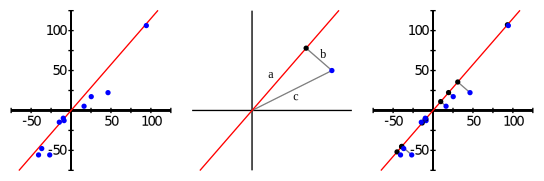
\includegraphics{PCA_spread}}
%\resizebox{!}{1.25in}{\includegraphics{PCA_rotated}} \hspace{0.1in} \resizebox{!}{1.25in}{\includegraphics{PCA_spread_distance}}  \hspace{0.1in} \resizebox{!}{1.25in}{\includegraphics{PCA_2_pc1_min}} 
    \caption{The principal component.}
    \label{F:PCA_pc}
  \end{center}
\end{figure}

\item Recall that the matrix (to two decimal places) $P =  \left[ \begin{array}{rr} - 0.66&-0.76\\ 0.76&0.66\end{array} \right]$ transforms the data set $X$ to a new data set $Y=PX$ whose covariance matrix is diagonal. Explain how the $x$-axis is related to the transformed data set $Y$. 
%Notice that $P$ looks like a rotation matrix, but is not exactly a rotation matrix. To understand what $P$ does to $X$, a plot of the original data from $X$ is shown with solid blue circles and a plot of the transformed data from $Y$ in solid magenta diamonds is at left in Figure \ref{F:PCA_P}. The form of the matrix $P$ looks similar to a rotation matrix, but is not exactly a rotation matrix. Show that $P$ is a combination of a rotation matrix (and find the rotation angle) and a reflection (and specifically identify the reflection). Explain how this relates to Figure \ref{F:PCA_P}. Also explain how the $x$-axis is related to the transformed data set $Y$. 
 
 \begin{figure}[ht]
  \begin{center}
  \resizebox{!}{2.0in}{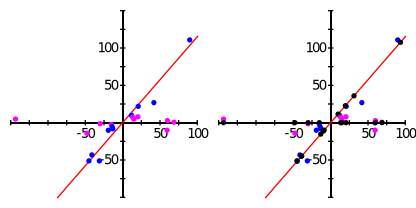
\includegraphics{PCA_P}}
%\resizebox{!}{2.0in}{\includegraphics{PCA_2_P_a}}  \hspace{0.5in} \resizebox{!}{2.0in}{\includegraphics{PCA_2_P}} 
    \caption{Applying $P$.}
    \label{F:PCA_P}
  \end{center}
\end{figure}


\ea

\end{pactivity}

The result of Project Activity \ref{act:PCA_max_min} is that we have reduced the problem from considering the data in a two-dimensional space to a one-dimensional space $E_{\lambda_1}$ where the most important aspect of the data is revealed. Of course, we eliminate some of the characteristics of the data, but the most important aspect is still included and highlighted. This is one of the important uses of PCA, data dimension reduction, which allows us to reveal key relationships between the variables that might not be evident when looking at a large dataset. 

The second eigenvector of $XX^{\tr}$ also has meaning. A picture of the eigenspace $E_{\lambda_2}$ corresponding to the smaller eigenvector $\lambda_2$ of $XX^{\tr}$ is shown in Figure \ref{F:PCA_second_pc}. The second eigenvector of $XX^{\tr}$ is orthogonal to the first, and the direction of the second eigenvector tells us the direction of the second most amount of  variance as can be seen in Figure \ref{F:PCA_second_pc}.
\begin{figure}[ht]
  \begin{center}
  \resizebox{!}{2.0in}{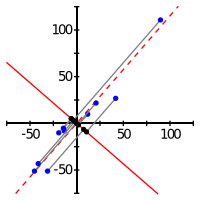
\includegraphics{PCA_second}} 
%\resizebox{!}{1.5in}{\includegraphics{PCA_2_second_pc}} 
    \caption{The second principal component.}
    \label{F:PCA_second_pc}
  \end{center}
\end{figure}


To summarize, the unit eigenvector for the largest eigenvalue of $XX^{\tr}$ indicates the direction in which the data has the greatest variance. The direction of the unit eigenvector for the smaller eigenvalue shows the direction in which the data has the second largest variance. This direction is also perpendicular to the first (indicating $0$ covariance). The directions of the eigenvectors are called the \emph{principal components} of $X$. The eigenvector with the highest eigenvalue is the first principal component of the data set and the other eigenvectors are ordered by the eigenvalues, highest to lowest. The principal components provide a new coordinate system from which to view our data -- one in which we can see the maximum variance and in which there is zero covariance. 

\begin{pactivity} \label{act:PCA_variances} We can use the eigenvalues of $XX^{\tr}$ to quantify the amount of variance that is accounted for by our projections. Notice that the points along the $x$-axis at right in Figure \ref{F:PCA_P} are exactly the numbers in the first row of $Y$. These numbers provide the projections of the data in $Y$ onto the $x$-axis -- the axis along which the data has its greatest variance.
\ba
\item Calculate the variance of the data given by the first row of $Y$. This is the variance of the data i the direction of the eigenspace $E_{\lambda_1}$. How does the result compare to entries of the covariance matrix for $Y$.


\item Repeat part (a) for the data along the second row of $Y$. 



\item The total variance of the data set is the sum of the variances. Explain why the amount of variance in the data that is accounted for in the direction of $E_{\lambda_1}$ is 
\[\frac{\lambda_1}{\lambda_1 + \lambda_2}.\]
Then calculate this amount for the SAT data. 

\ea

\end{pactivity}

In general, PCA is most useful for larger data sets. The process is the same. 
\begin{itemize}
\item Start with a set of data that forms the rows of an $m \times n$ matrix. We center the data by subtracting the mean of each row from the entries of that row to create a centered data set in a matrix $X$. 
\item The principal components of $X$ are the eigenvectors of $XX^{\tr}$, ordered so that they correspond to the eigenvalues of $XX^{\tr}$ in decreasing order. 
\item Let $P$ be the matrix whose rows are the principal components of $X$, ordered from highest to lowest. Then $Y = PX$ is suitably transformed to identify the important aspects of the data. 
\item If $\lambda_1$, $\lambda_2$, $\ldots$, $\lambda_n$ are the eigenvalues of $XX^{\tr}$ in decreasing order, then the amount of variance in the data accounted for by the first $r$ principal components is given by
\[\frac{\lambda_1+\lambda_2 + \cdots + \lambda_r}{\lambda_1+\lambda_2 + \cdots + \lambda_n}.\]
\item The first $r$ rows of $Y=PX$ provide the projection of the data set $X$ onto an $r$-dimensional space spanned by the first $r$ principal components of $X$.  
\end{itemize}


\begin{pactivity} \label{act:PCA_4D_SAT} Let us now consider a problem with more than two variables. We continue to keep the data set small so that we can conveniently operate with it. Table \ref{T:PCA_SAT} presents additional information from ten states on four attributes related to the SAT -- Participation rates, Evidence-Based Reading and Writing (EBRW) score, Math score, and average SAT score. Use technology as appropriate for this activity. 
\begin{table}[ht]
\begin{center}
\setlength{\tabcolsep}{3pt}
\begin{tabular}{lcccccccccc} 
State			&$1$	 &$2$ &$3$ &$4$ &$5$ &$6$ &$7$ &$8$ &$9$ &$10$ \\ \hline
Rate 	&$6$ &$60$ &$97$ &$100$ &$64$ &$99$ &$4$ &$23$ &$79$ &$70$ \\ 
EBRW		&$595$ &$540$ &$522$ &$508$ &$565$ &$512$ &$643$ &$574$ &$534$ &$539$ \\
Math			&$571$ &$536$ &$493$ &$493$ &$554$ &$501$ &$655$ &$566$ &$534$ &$539$ \\
SAT			&$1166$ &$1076$ &$1014$ &$1001$ &$1120$ &$1013$ &$1296$ &$1140$ &$1068$ &$1086$ 
\end{tabular}
\caption{SAT data.}
\label{T:PCA_SAT}
\end{center}
\end{table}
\ba
\item Determine the centered data matrix $X$ for this data set.


\item Find the covariance matrix for this data set. Round to four decimal places. 


\item Find the principal components of $X$. Include at least four decimal places accuracy. 

\item How much variation is accounted for in the data by the first principal component? In other words, if we reduce this data to one dimension, how much of the variation do we retain? Explain.

\item How much variation is accounted for in the data by the first two principal components? In other words, if we reduce this data to two dimensions, how much of the variation do we retain? Explain.


\ea

\end{pactivity}

We conclude with a comment. A reasonable question to ask is how we interpret the principal components. Let $P$ be an orthogonal matrix such that $PCP^{\tr}$ is the diagonal matrix with the eigenvalues of $C$ along the diagonal, in decreasing order. We then have the new perspective $Y = PX$ from which to view the data. The first principal component $\vp_1$ (the first row of $P$) determines the new variable $\vy_1 = [y_i]$ (the first row of $Y$) in the following manner. Let $\vp_1 = [p_i]^{\tr}$ and let $\vc_i$ represent the columns of $X$ so that $X = [\vc_1 \ \vc_2 \ \vc_3 \ \cdots \ \vc_{20}]$.  Recognizing that 
\[PX =  \left[ \renewcommand{\arraystretch}{1.2} \begin{array}{c} \vp_1^{\tr} \\ \vp_2^{\tr} \\ \vp_3^{\tr} \\ \vp_4^{\tr} \\\vp_5^{\tr} \\ \vp_6^{\tr} \end{array} \right]  [\vc_1 \ \vc_2 \ \vc_3 \ \cdots \ \vc_{20}],\]
%\left[ \begin{array}{c} \vx_1^{\tr} \\ \vx_2^{\tr} \end{array] \right]
we have that 
\[y_i = \vp_1^{\tr} \vc_i.\]
That is,
\[\vy_1 = [\vp_1^{\tr}\vc_1 \ \vp_1^{\tr} \vc_2 \ \vp_1^{\tr} \vc_3 \ \cdots \ \vp_{1}^{\tr} \vc_{20}].\]
So each $y_i$ is a linear combination of the original variables (contained in the $\vc_i$) with weights from the first principal component. The other new variables are obtained in the same way from the remaining principal components. So even though the principal components may not have an easy interpretation in context, they are connected to the original data in this way. By reducing the data to a few important principal components -- that is, visualizing the data in a subspace of small dimension -- we can account for almost all of the variation in the data and relate that information back to the original data.  




